% REMEMBER TO SET LANGUAGE!
\documentclass[a4paper,10pt,english]{article}
\usepackage[utf8]{inputenc}
\usepackage[english]{babel}
% Standard stuff
\usepackage{amsmath,graphicx,babel,varioref,verbatim,amsfonts}
% colors in text
\usepackage[usenames,dvipsnames,svgnames,table]{xcolor}
% Hyper refs
\usepackage[framestyle=none,framefit=yes,heightadjust=all,framearound=all]{floatrow}    
\floatsetup[figure]{style=Boxed,framearound=all}
\usepackage{fancyhdr}
\usepackage[colorlinks]{hyperref}

% Document formatting
\setlength{\parindent}{0mm}
\setlength{\parskip}{1.5mm}
%\setcounter{section}{-1} Hvis du vil ha 0 som første avsnitt
\numberwithin{figure}{section} 
\numberwithin{table}{section}
\numberwithin{equation}{section}

%Color scheme for listings
\usepackage{textcomp}
\definecolor{listinggray}{gray}{0.9}
\definecolor{lbcolor}{rgb}{0.9,0.9,0.9}

%Listings configuration
\usepackage{listings}
\lstset{
	backgroundcolor=\color{lbcolor},
	tabsize=4,
	rulecolor=,
	language=python,
        basicstyle=\scriptsize,
        upquote=true,
        aboveskip={1.5\baselineskip},
        columns=fixed,
	numbers=left,
        showstringspaces=false,
        extendedchars=true,
        breaklines=true,
        prebreak = \raisebox{0ex}[0ex][0ex]{\ensuremath{\hookleftarrow}},
        frame=single,
        showtabs=false,
        showspaces=false,
        showstringspaces=false,
        identifierstyle=\ttfamily,
        keywordstyle=\color[rgb]{0,0,1},
        commentstyle=\color[rgb]{0.133,0.545,0.133},
        stringstyle=\color[rgb]{0.627,0.126,0.941}
        }
        
%User settings
\newcounter{subproject}
\renewcommand{\thesubproject}{\alph{subproject}}
\newenvironment{subproj}{
\begin{description}
\item[\refstepcounter{subproject}(\thesubproject)]
}{\end{description}}
\newcommand{\HRule}{\rule{\linewidth}{0.5mm}}
\newcommand{\eqs}{\begin{equation}}
\newcommand{\eqf}{\end{equation}}


%Other
\usepackage{geometry}
\usepackage{booktabs}
\newcommand{\shaderow}{\rowcolor{gray!20}[2pt][2pt]}
\usepackage[boxed,linesnumbered,lined]{algorithm2e}

%Lettering instead of numbering in different layers
%\renewcommand{\labelenumi}{\alph{enumi}}
%\renewcommand{\thesubsection}{\alph{subsection}}



\begin{document}
%Header
\pagestyle{fancy}
\renewcommand{\sectionmark}[1]{\markright{#1}{}}

\pagestyle{fancy}
\renewcommand{\sectionmark}[1]{\markright{\thesection\ #1}}

\fancyhf{}
%Header
%\rhead{\fancyplain{}{ NAVN PÅ PROSJEKT}} % predefined ()
\lhead{\fancyplain{}{\rightmark }} % 1. sectionname, 1.1 subsection name etc
\cfoot{\fancyplain{}{\thepage}}


%Forside
\begin{titlepage}
\begin{center}

% Upper part of the page. The '~' is needed because \\
% only works if a paragraph has started.

\includegraphics[width=0.4\textwidth]{forside.jpg}~\\[1cm]

\textsc{\LARGE Project 3}\\[1.5cm]

\textsc{\Large FYS3150 - Computational physics}\\[0.5cm]

% Title
\HRule \\[0.4cm]
{ \huge \bfseries Quantum dots \\[0.4cm] }

\HRule \\[1.5cm]

% Author and supervisor
\begin{minipage}{0.4\textwidth}
\begin{flushleft} \large
\emph{Author:}\\
Vidar \textsc{Skogvoll}
\end{flushleft}
\end{minipage}
\begin{minipage}{0.4\textwidth}
\begin{flushright} \large
\emph{ } \\
 \textsc{ }
\end{flushright}
\end{minipage}

\vfill

% Bottom of the page
{\large \today}

\end{center}
\end{titlepage}
\setcounter{page}{2}

\begin{abstract}
Here is a short summary of the project.
\end{abstract}

\hypersetup{linkcolor=black}
\tableofcontents 
\hypersetup{linkcolor=red}
\clearpage




\section{Introduction}
Quantum mechanics is an exciting field. 








\section{Theory}
Here is all the theory needed to understand the project.


\subsection{The numerical foundation}
This is the section explaining the numerical theory upon which the project is built. 

\subsubsection{Monte Carlo simulations}
A Monte Carlo simulation is a way of solving a mathematical or physical problem by generating a random
(or pseudorandom
\footnote
{No electronic random number generator of today is truly random. 
The sequence of numbers generated will repeat itself after a long period. 
These periods however, are increadibly long and we will for this report 
consider the random number generators to be truly random.})
sequence of numbers and evaluating some quantity on the assumption that our the random sequence of numbers is representative of the domain from which the quantity is evaluated.
An example is evaluating the area of the unit circle by randomly placing points in a $[-1,1] \times [-1,1] $ grid and find the fraction points whose distance to the origin is $\leq 1$ and multiply this fraction by the area of the grid (i.e. $4$).
Such a simple Monte Carlo simulation can give the result as shown in figure \ref{fig:Monte_Carlo_Illustration}.

\begin{figure}[h!]
        \centering 
        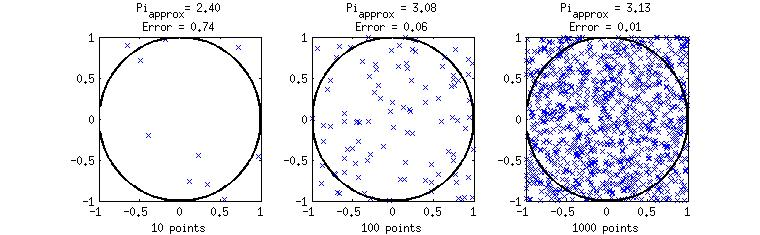
\includegraphics[width=\textwidth]{Monte_Carlo_Illustration.jpg}
        \caption{The results from a very simple Monte Carlo simulation of 
        estimating the circle constant $\pi$. 
        The precision increases with the number of points.}
        \label{fig:Monte_Carlo_Illustration}
\end{figure}

However, the method is not confined to this sort of problem, but can be applied to a variety of mathematical and physical problems. 
In this report, the method, through the Metropolis algorithm (see section \ref{sec:theory_metropolis}) has been applied to a quantum mechanical system.

\subsubsection{Importance sampling}

Sometimes, functions are more important in certain domains.
When we use a Monte Carlo approach to evaluate a quantity on such a function we can improve the method significantly by ensuring that the probability distribution from which we choose our random values reflect the parts where the function is important.
We do of course have to remember that our function lives on its whole domain, so to not get a biased result, we need to weigh our result with respect to the probability function we have chosen. 
This is called importance sampling. 
\textbf{INSERT EXAMPLE HERE}

\subsubsection{Metropolis algorithm} \label{sec:theory_metropolis}

The metropolis algorithm is a Monte Carlo method discovered in \textbf{???} by \textbf{???}. 

\subsection{The physical system}
This is the section explaining the physics of the system. 

\subsubsection{Quantum mechanics}

\subsubsection{Discretization}

\subsubsection{The virial theorem}








\section{Method}
This is the section explaining what has been done.


\subsection{Subsection}
These will become apparent as the work boils down. 








\section{Results and discussion}
Section listing results and discussing them. 


\subsection{Subsection}
The same as the method section. 








\section{Conclusion}

\end{document}